\documentclass[12pt]{article}
\usepackage[margin=1in]{geometry}
\usepackage{graphicx}
\usepackage{titlesec}
\usepackage{parskip}
\usepackage{float}
\usepackage{hyperref}

\title{\textbf{Final Report} \\
CPSC 6820: Embedded Systems Prototyping \\
Spring 2025 \\
\Large Team Happy Pets}
\author{
Sriram Vishnubhotla (\texttt{svishnu@clemson.edu}) \and
Logan Swoyer (\texttt{lswoyer@clemson.edu}) \and
Jacob Sorber (\texttt{jsorber@clemson.edu})
}
\date{April 25, 2025}

\begin{document}

\maketitle

\section{Project Summary}
In this project, we build an automatic pet feeder with flexible scheduling and wireless connectivity. The device includes a small display and a knob for navigating menus, setting feeding times, and adjusting portion sizes. We implement system clock configuration and Wi-Fi support to enable automatic time synchronization and remote schedule updates. When connected to Wi-Fi, the feeder syncs its internal clock and retrieves feeding schedules from a remote server, allowing future integration with mobile applications. The feeder includes a dispensing area with space underneath to place a bowl, ensuring food is delivered directly to the container.
\section{Project Description and Implementation}
Our current implementation consists of a functional prototype assembled using basic materials. The main body is made from a cardboard box, while a reused plastic bottle serves as the food storage container. A cardboard flap attached to the bottle's opening acts as a gate that opens and closes to dispense food. This mechanism is driven by a small servo motor.

We use M5Stack's DinMeter as the core control unit, which features an Espressif ESP32-S3 microcontroller. The DinMeter also includes a rotary encoder knob, a display, and a buzzer. A proximity-based ultrasonic sensor is mounted beneath the container lid to estimate the remaining food level inside the bottle.

The user interface is built using LVGL 9 and presented as a scrollable list of menu items. Users interact with the menus using the built-in knob to configure settings such as the system clock, check Wi-Fi status, view live sensor readings, and test output devices like the servo motor and buzzer.

All firmware is developed using Espressif's ESP-IDF framework, which provides a comprehensive set of APIs for FreeRTOS-based development and includes support for peripherals, networking, and device drivers.
\subsection{Changes}
We initially planned to use the MSP430 development board as the main controller and an ESP32 module solely for Wi-Fi connectivity. However, as we evaluated the capabilities of the ESP32, we realized it was sufficiently powerful to handle both control logic and network communication on its own. This led us to consider the ESP32-C3 development board as a simpler alternative. Eventually, we transitioned to using the M5Stack DinMeter, a compact module that integrates an ESP32-S3 microcontroller, a display, a rotary knob, and a buzzer in a single enclosed unit. This shift allowed us to consolidate multiple components into a single package, simplifying both hardware integration and enclosure design.

While the DinMeter offered convenience and a clean form factor, it introduced some unexpected limitations. Its small plastic enclosure restricts access to GPIO ports, and the available ports are exposed through a proprietary Grove connectors with a non-standard 2.0mm pitch. To connect our external sensors and motor, we had to remove the proprietary connectors and manually solder wires, which resulted in a less reliable and messier hardware setup. On the mechanical side, we initially considered 3D printing the enclosure but had to settle for cardboard due to time constraints and circumstances. The cardboard proved flimsy and structurally weak, especially when combined with a manually mounted servo mechanism. We also faced delays in finalizing the actuator. Although we considered linear actuators, we ultimately chose a small SG90 servo motor based on availability, cost, and the availability of resources online for rotational actuators. The servo drives a cardboard flap used to dispense food, which presented alignment and strength challenges due to the softness of the material.
\subsection{Software}
I developed the firmware for this device using Espressif's ESP-IDF, a FreeRTOS-based framework that provides C APIs and drivers for peripherals, timers, networking, and other components of the ESP32 platform. The DinMeter initially shipped with Arduino-compatible firmware and we wrote the initial code in Arduino-style C++ as well, but I chose to reimplement all logic in standard C using ESP-IDF due to some complications and to have full control over scheduling and hardware initialization and to make use of ESP-IDF's drivers.

The codebase is organized around a hardware configuration header file, which defines GPIO assignments, I2C addresses for connected sensors, display parameters, and actuator timing values. These macros are used consistently throughout the code to simplify maintenance. At startup, I initialize the I2C interface using ESP-IDF's master bus driver and register the connected ultrasonic sensor. I originally planned to use a weight sensor based on the HX711 to measure dispensed food portions, but the sensor consistently returned erratic values---swinging between extreme readings without stability. Despite verifying the wiring, firmware, and initialization logic, I could not obtain reliable data, so I decided to omit the weight sensor from the final implementation.

For actuator control, I used the ESP32's motor control PWM (MCPWM) module. This involved configuring a timer, operator, comparator, and generator to produce PWM signals. The servo motor's angle is translated into a specific pulse width and passed to the comparator module. This setup reliably actuates a cardboard flap used to dispense food.

The user interface was implemented using LVGL version 9. I used a scrollable list layout that provides access to key functions including system clock settings, feeding schedule configuration, peripheral testing, and real-time sensor data. The DinMeter's display required manual configuration to handle its cropped resolution: I defined a larger virtual resolution than physically present and applied a crop window to match the actual dimensions.

The scheduling system is central to the application. When a user adds a schedule, the system stores it in an in-memory array along with the time in minutes from midnight. A timer is then set to trigger at the closest upcoming scheduled time. Each time a schedule is added, edited, or completed, the nearest future schedule is calculated and the timer re-armed accordingly. The logic includes wraparound handling for events past midnight. Each timer trigger invokes a callback, which executes the corresponding dispensing action.
\subsection{Hardware}
We use the following hardware components in our automatic pet feeder:

\begin{table}[h]
    \centering
    \begin{tabular}{p{0.3\textwidth} p{0.65\textwidth}}
        \hline
        \textbf{Component}                    & \textbf{Description}                                                                                                        \\
        \hline
        M5Stack DinMeter                      & Integrated module with ST7789V2 LCD display, ESP32-S3 microcontroller, rotary encoder, buzzer, and RTC8563 real-time clock. \\
        M5Stack I2C Weight Unit (HX711-STM32) & Load cell amplifier with built-in STM32 for weight measurement (unused due to unreliable readings).                         \\
        M5Stack Ultrasonic Sensor (RCWL-9620) & I2C-based proximity sensor for measuring food level in the storage container.                                               \\
        SG90 Micro Servo 9g                   & Compact 6 V-compatible servo motor used to actuate the dispensing flap.                                                     \\
        6 V DC Power Adapter                  & External power supply providing stable 6 V to the entire system.                                                            \\
        \hline
    \end{tabular}
    \caption{Hardware components}
\end{table}

\subsection{Prototype Pictures}
\begin{figure}[H]
    \centering
    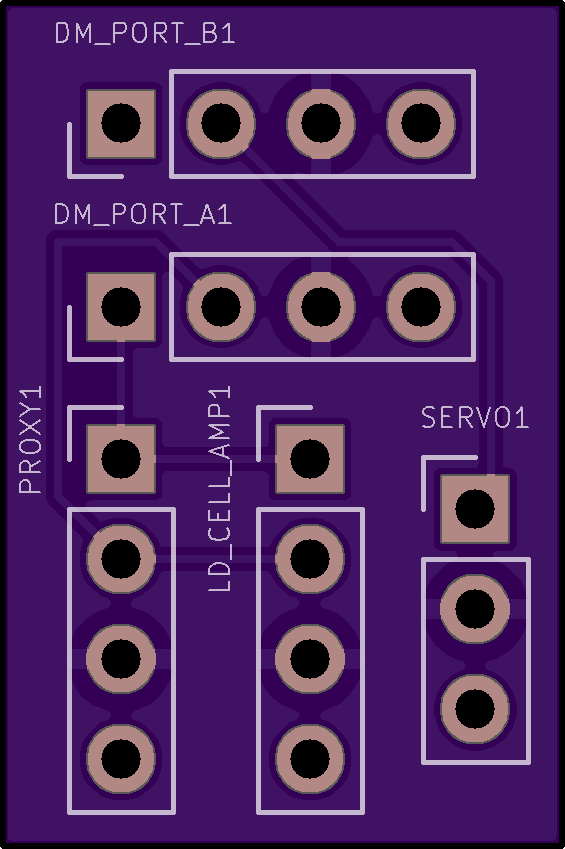
\includegraphics[height=0.5\textheight]{board-front.png}
    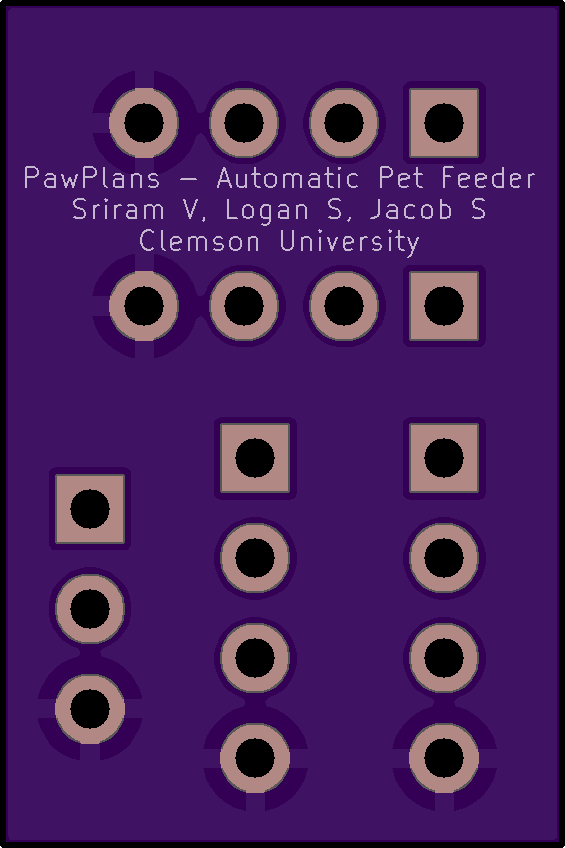
\includegraphics[height=0.5\textheight]{board-back.png}
    \caption{OSH Park PCB preview}
\end{figure}
\begin{figure}[H]
    \centering
    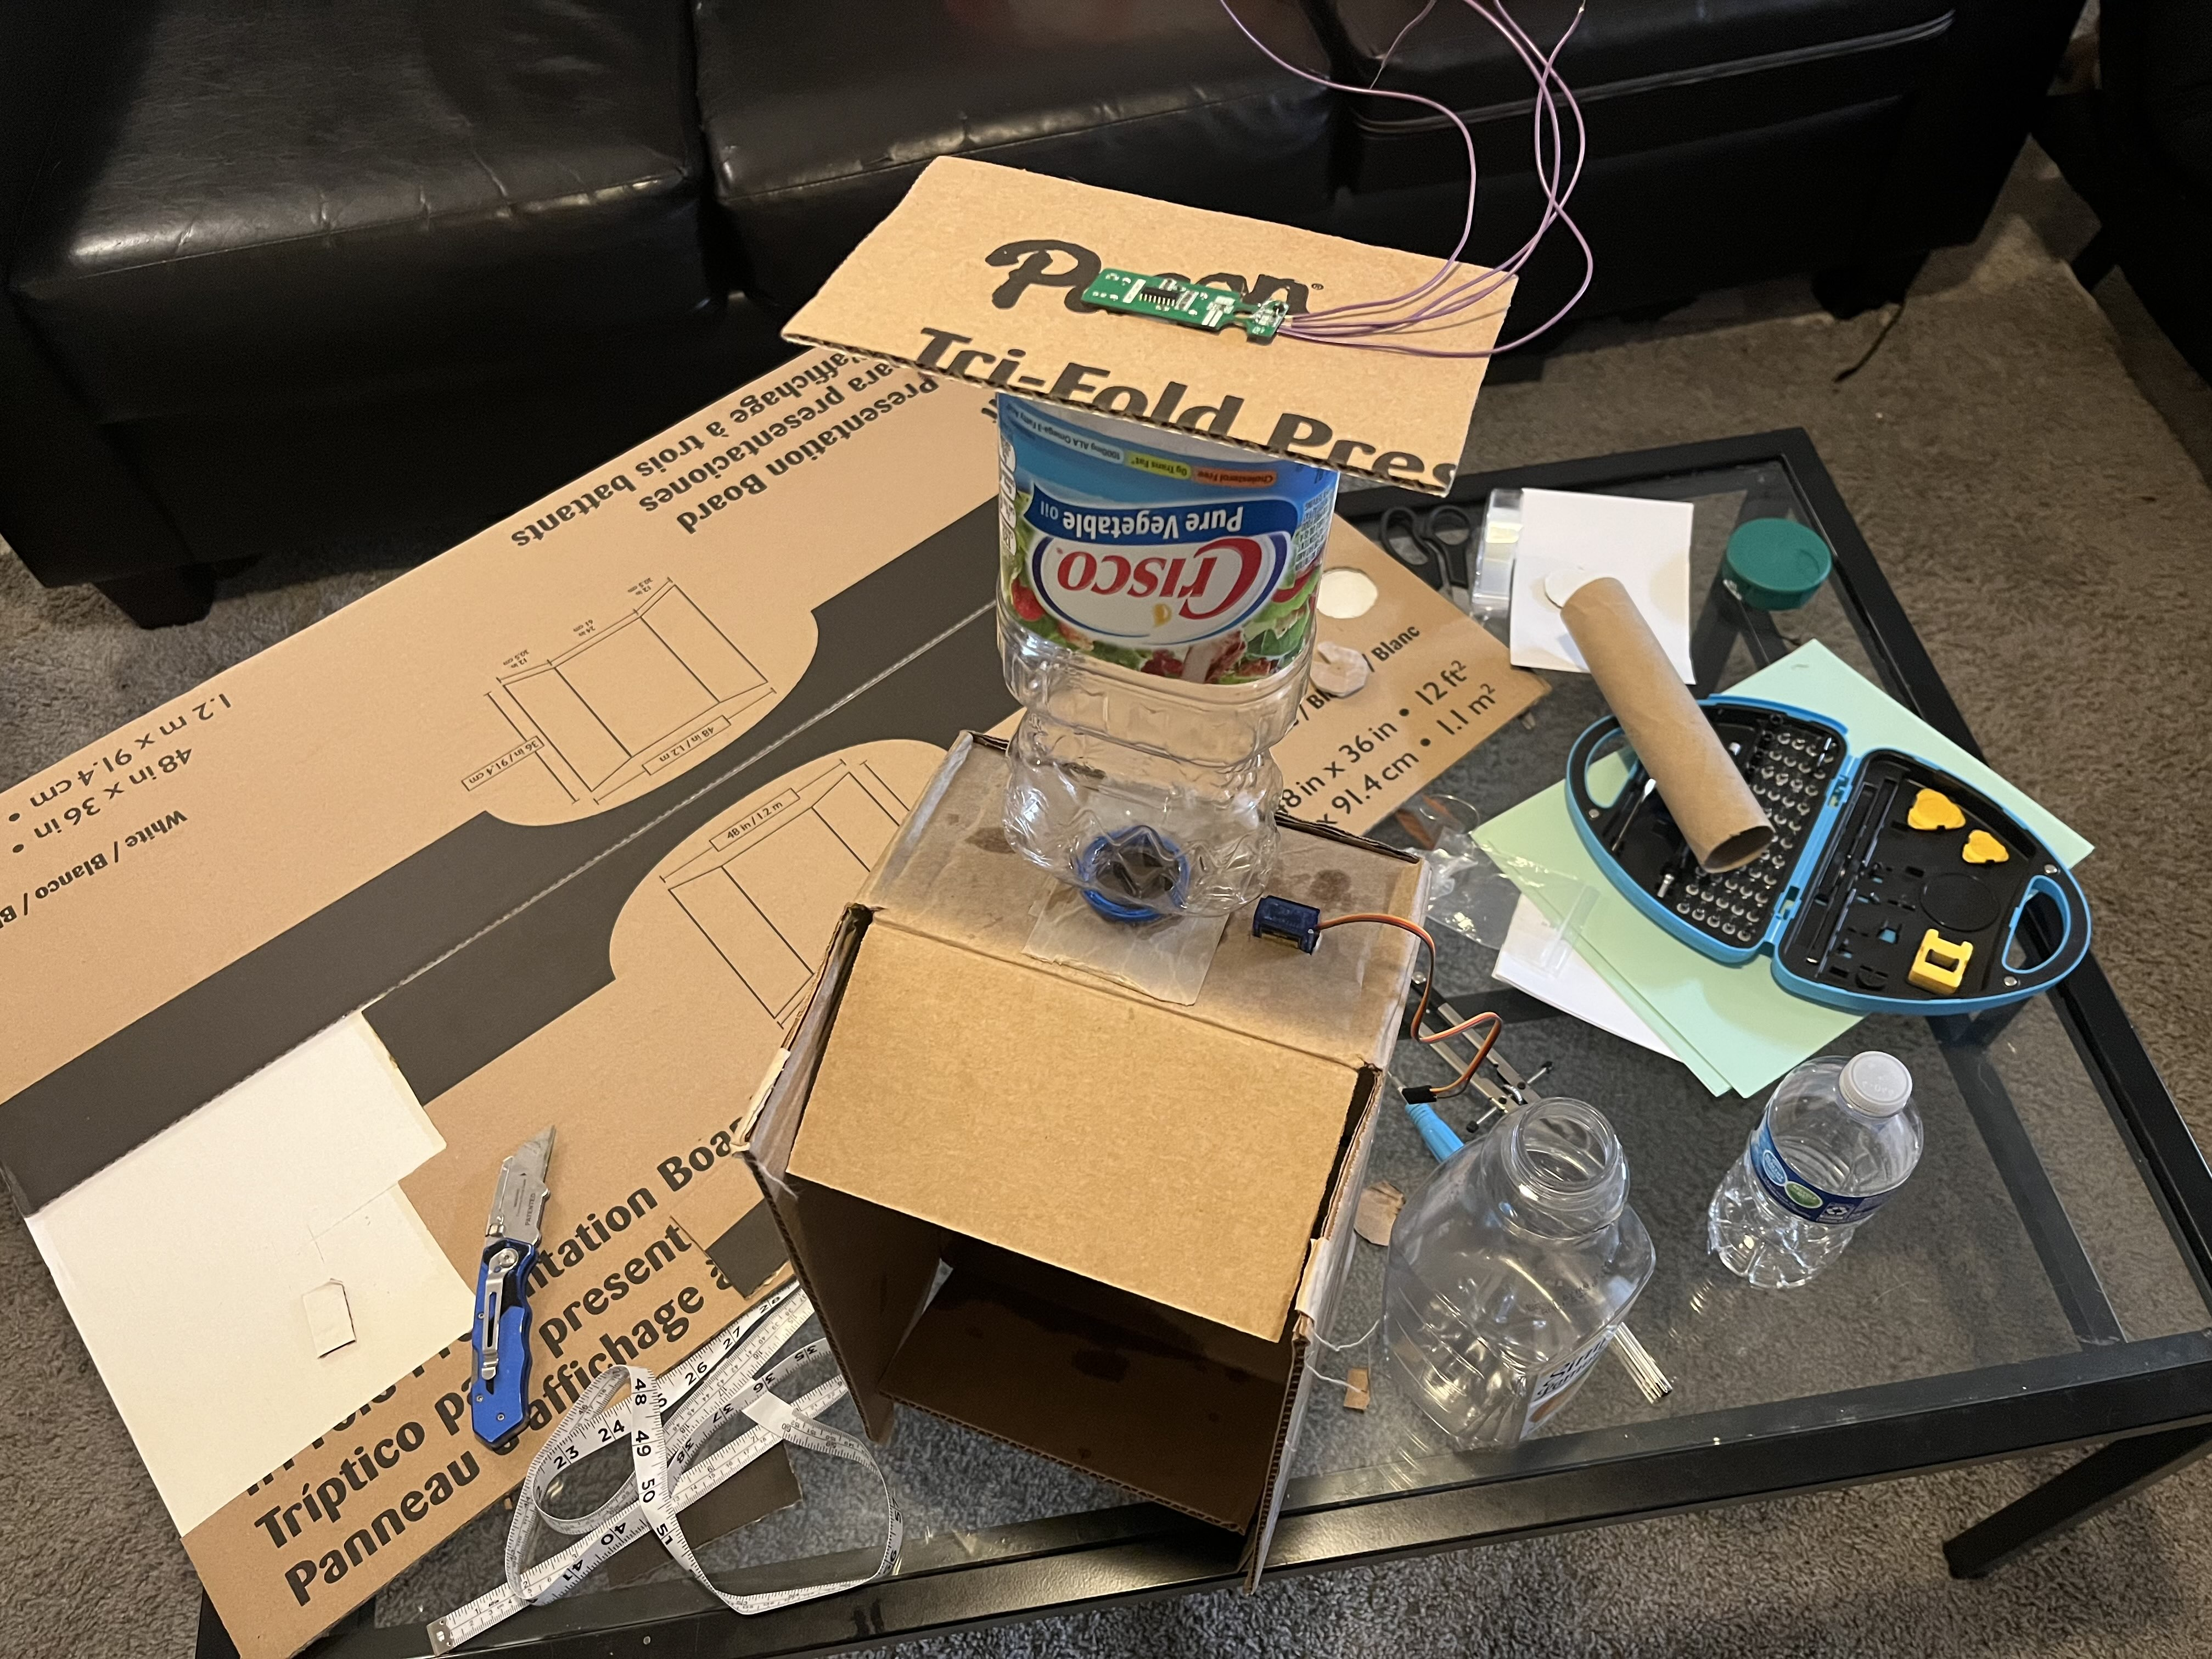
\includegraphics[width=0.45\textwidth]{chassis-wip.jpg}
    \includegraphics[width=0.45\textwidth]{chassis-basic.jpg}
    \caption{Device chassis WIP and a basic prototype}
\end{figure}
\begin{figure}[H]
    \centering
    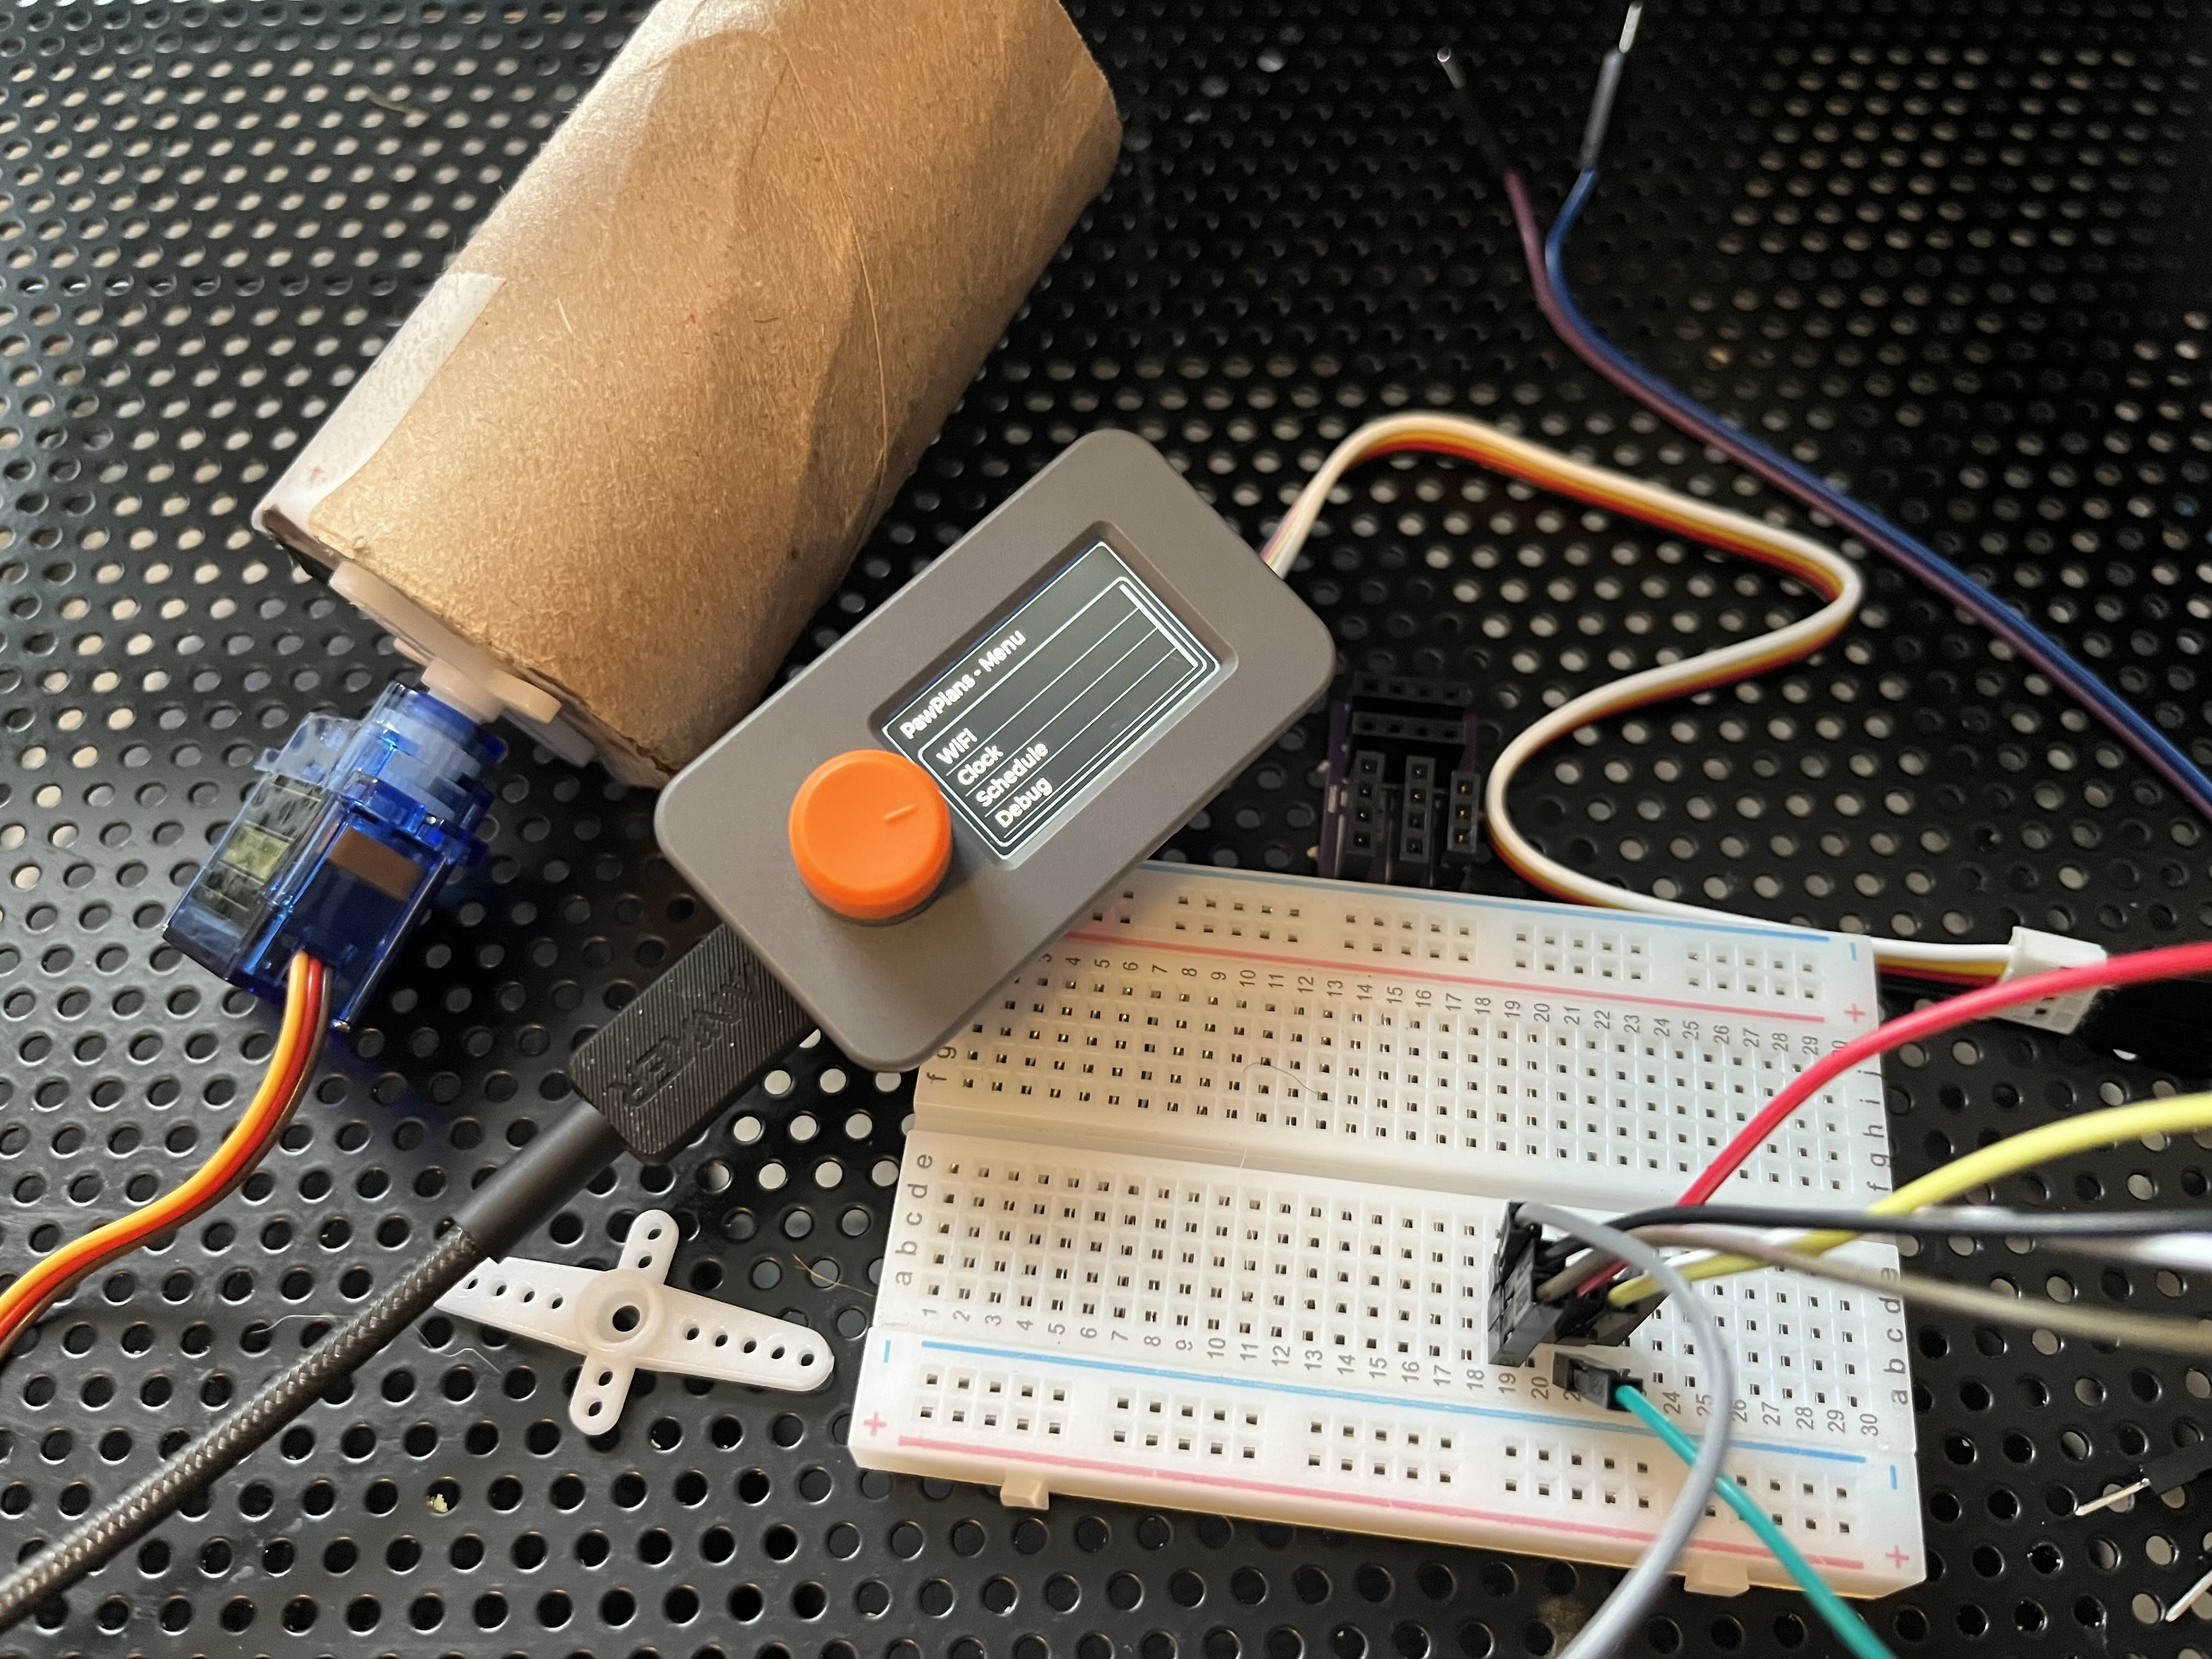
\includegraphics[width=0.8\textwidth]{parts.jpg}
    \caption{Early trials with servo, using a rotating drum instead of a flap}
\end{figure}


\subsection{Challenges and Team Work}
Throughout the course of the project, we experienced several challenges that needed teamwork and coordination to manage. One significant factor for delay was determining the torque requirements for the servo motor, as it was challenging to estimate how much weight the motor needed to bear and as the motors are expensive. Additionally, the design of the pet feeder's body proved to be more complicated to build with cardboard. While we had originally planned to 3D model the design, I ultimately resorted to using cardboard for the final delivery, which presented its own challenges.

In terms of teamwork, coordination was a challenge. Scheduling conflicts due to classes was a challenge in making consistent progress. I am thankful for Logan for working with me throughout the course but unfortunately his withdrawal from the course left me to handle the majority of the work on my own, especially since I had been working on a firmware rewrite in C. This shift affected my motivation and introduced additional pressure, as I had to take over all aspects of the project, including checking and assembling the components and working on the body of the device. I also encountered another unfortunate setback when I accidentally uploaded an incomplete version of the Gerber files to the board printing service, which resulted in an improperly routed PCB, which I only realized when soldering the board. As a result, I had to fall back on using a breadboard for connections. Furthermore, the proprietary connectors in some components required manual modifications, including desoldering the ports and soldering wires in their place.

Despite these obstacles, I think we made a fair amount of progress overall and learned a great deal from the experience.

\section{Resources}
Source code for the project can be found on \href{https://github.com/openbraces/CPSC-6820}{GitHub} at this path: \texttt{CPSC-6820/PawPlans}.
The following resources were used in the development of the automatic pet feeder:
\begin{itemize}
    \item ESP-IDF Documentation: Espressif provides great documentation with examples, guides and API documentation.
    \item LVGL 9 Documentation: Documentation for the LVGL graphics library helped implement the user interface.
    \item SG90 Servo Datasheet: The servo datasheet was used to determine control pulse widths, power requirements, and angle limits for the dispensing mechanism.
    \item \href{https://www.instructables.com/Cereal-Dispenser-made-From-a-Cereal-Box/}{Instructables} and \href{https://www.makersgeneration.net/single-post/learn-electronics-for-beginners-how-to-make-a-diy-pet-feeder-with-an-arduino-board}{Makers Generation} provided ideas for the physical design of the feeder, especially using household materials.
    \item Adafruit and SparkFun Tutorials: General learning guides and posts helped during early prototyping and in general during the course.
\end{itemize}

\section{Class Feedback}

\subsection{Challenges}
This course has been engaging and provided valuable experience to me. It offered a practical introduction to embedded systems and helped me gain confidence working with low-level hardware. While the project itself was challenging, many of the setbacks I encountered---especially toward the end---could likely have been avoided by following the recommended timeline more closely. In hindsight, choosing a less ambitious project might have allowed us to spend more time polishing the result rather than trying to build a fully featured device within the course timeline. That said, I do not think the course itself needs significant changes. The structure, pacing, and support resources were all well-designed. If anything, I hope for the return of the 8000-level follow-up course to explore advanced topics in embedded systems in more depth, since this course effectively lays the groundwork.

\subsection{General Comments}

This has been my favorite class so far due to its interactive structure and the open, student-friendly environment. The professor was friendly, provided helpful guidance, and encouraged team discussions during the classes. We have had technical issues with Buffet, but the transition to GitLab should hopefully improve the experience for future students.
\end{document}
